\section{User Interface}
This section will look at how each of the designed UI aspects were implemented. UI implementation made use of controllers, which were responsible for conducting database interactions and returning the relevant view, along with HTML, CSS and Javascript for page structure, design and usability. Implementation for different UI components was identical to the concept designs discussed in Chapter \ref{Chapter:Design}.

\subsection{Navigation}
Figure \ref{fig:NavImplementation} shows the implemented navigation bars for unauthorised and unauthorised users. Users are able to navigate to the pages represented by each of the icons on the navigation bar. 

\begin{figure}[H]
	\centering
	\begin{subfigure}{1\linewidth}
		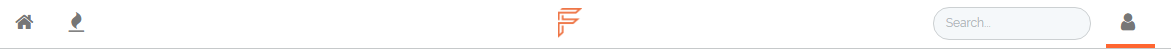
\includegraphics[width=1\textwidth]{Images/Design/nav-unauthorised}
		\caption{Guest}
		\label{fig:NavUnauth}
	\end{subfigure}
	\begin{subfigure}{1\linewidth}
		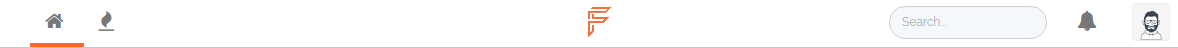
\includegraphics[width=1\textwidth]{Images/Design/nav-authorised}
		\caption{Authorised User}
		\label{fig:NavAuth}
	\end{subfigure}
	\caption{Fidelis navigation bar for (a) unauthorised and (b) authorised users}
	\label{fig:NavImplementation}
\end{figure}

\subsubsection{Links}
Routes for each of the icons are populated using the \textit{LayoutComposer} class, which is a class method that is called whenever the Layout view is rendered \cite{Laravel:Views}. The navigation bar is rendered in the Layout view. Depending on whether the user is authorised or not, the composer returns the title, icon name, route and CSS properties of the relevant icon. Figure \ref{fig:LayoutComposerNav} shows the navigation options for user and application navigation.

\begin{figure}[H]
\centering
\begin{subfigure}[b]{1\linewidth}
	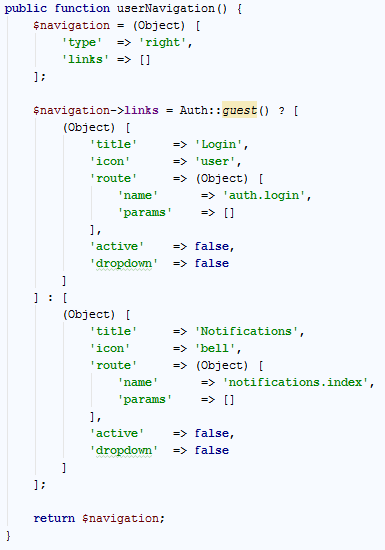
\includegraphics[width=1\textwidth]{Images/Implementation/UserNavigation}
	\caption{}
	\label{fig:UserNavigation}
\end{subfigure}
\begin{subfigure}[b]{1\linewidth}
	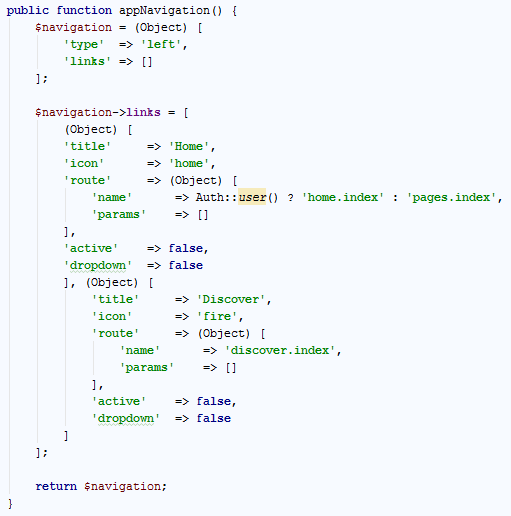
\includegraphics[width=1\textwidth]{Images/Implementation/AppNavigation}
	\caption{}
	\label{fig:AppNavigation}
\end{subfigure}
\caption{Rendering options for (a) user and (b) application navigation}
\label{fig:LayoutComposerNav}
\end{figure}

\subsubsection{Search}
The search bar allows users to enter a query term, and any user or tag matching this search term is retrieved. Using jQuery and JSON, it is possible to live-update the results from the supplied query term and display them to the user. Doing this removes the need to re-direct the user to a separate page which displays the search results to them. An API call to the \textit{SearchController} is made, in which all users and tags matching the query term are retrieved and returned to the view as a JSON object. Figure \ref{fig:SearchController} shows the retrieval of results that match the search term.

\begin{figure}[H]
\centering
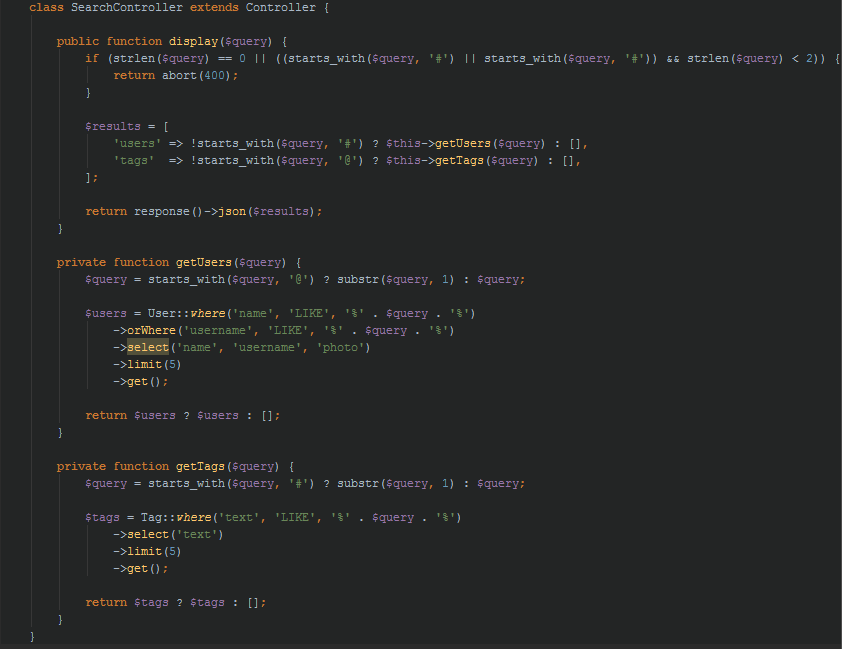
\includegraphics[width=1\textwidth]{Images/Implementation/SearchController}
\caption{Processing of query term performed in \textit{SearchController}}
\label{fig:SearchController}
\end{figure}

It is also possible to search specifically for a user or tag by preceding the query term with a \textbf{@} or \textbf{\#} respectively. Doing this restricts the results returns from the search to just users or tags. In Figure \ref{fig:SearchResults} we can see the implemented search bar, showing the results of providing ``H'' as a query term.

\begin{figure}[H]
\centering
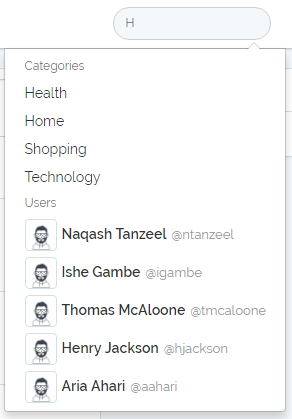
\includegraphics[height=2in]{Images/Implementation/SearchResults}
\caption{Results from searching for the term ``H''}
\label{fig:SearchResults}
\end{figure}

\subsection{Authentication}
Laravel provides built-in functionality for handling user authentication. With this, a number of controllers are available that manage authentication for user login, registration and password recovery \cite{Laravel:Authentication}. By executing the \textit{php artisan make:auth} command, all views and controllers related to user authentication are generated. This command also generates the routes required to navigate to the views, and access controller functionality.

\subsubsection{Registration}
The registration page, shown in Figure \ref{fig:RegisterPage}, collects the users' name, email address, username, date of birth, password, and also asks the user to agree with the Fidelis terms of service. If the user provides all the required fields, they are re-directed to the home page. The post-authentication redirection location can be modified in the \textit{RegisterController}.

\begin{figure}[H]
\centering
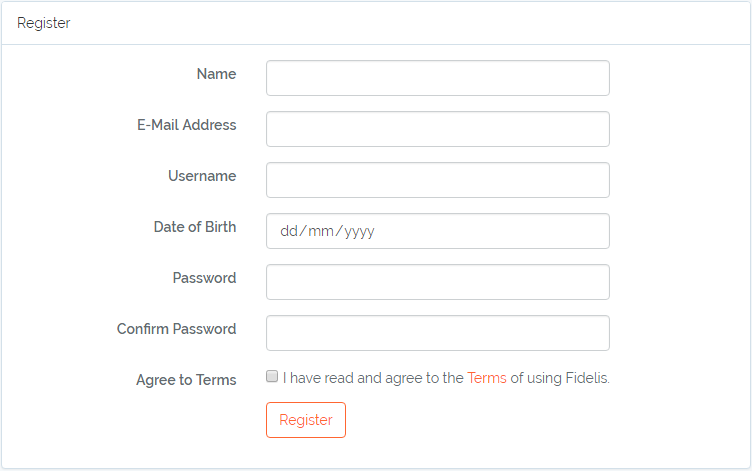
\includegraphics[height=2in]{Images/Design/register-page}
\caption{Registration page}
\label{fig:RegisterPage}
\end{figure}

In addition to the redirection location, the \textit{RegisterController} contains \texttt{validator()} and \texttt{create()} functions. Before the user is redirected to the home page on successful authentication, the controller first applies a set of validation rules specified in the validator (Figure \ref{fig:RegValidation}) which must be verified before the user is authenticated. If validation is correct, the new user is created with the \texttt{create()} function and authenticated (Figure \ref{fig:register-controller}), leading to successful redirection.

\begin{figure}[H]
\centering
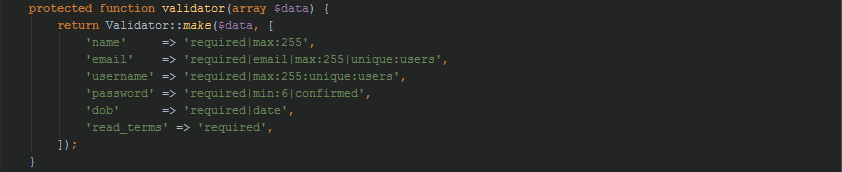
\includegraphics[width=\textwidth]{Images/Implementation/RegisterValidation}
\caption{Validation rules applies to fields supplied by user on the Registration page}
\label{fig:RegValidation}
\end{figure}

\subsubsection{Login}
The login page, shown in Figure \ref{fig:LoginPage}, requests the users' email address and password. Similarly to registration, users who are successfully authenticated are redirected to the home page. All authentication functionality is handled by the pre-built \textit{LoginController}. If incorrect account credentials are provided, authentication is unsuccessful.

\begin{figure}[H]
\centering
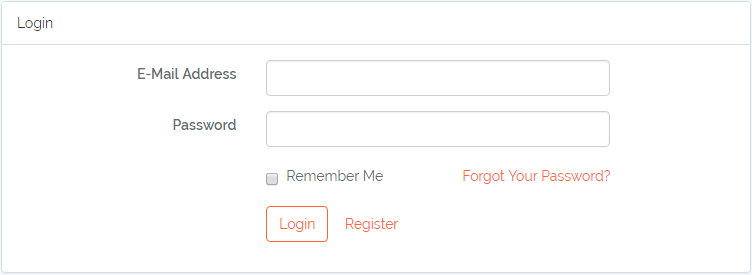
\includegraphics[height=1.5in]{Images/Design/login-page}
\caption{Log-in page}
\label{fig:LoginPage}
\end{figure}

\subsubsection{Password Reset}
The password reset page, shown in Figure \ref{fig:PasswordReset} allows users to reset their passwords if they have forgotten their account credentials. By navigating to this page, users can submit a form containing their email addressing. Submission of this form will prompt the \textit{ResetController}, which handles password resetting using pre-built functionality, to send a password reset link to the provided email address if an account exists for that address.

\begin{figure}[H]
\centering
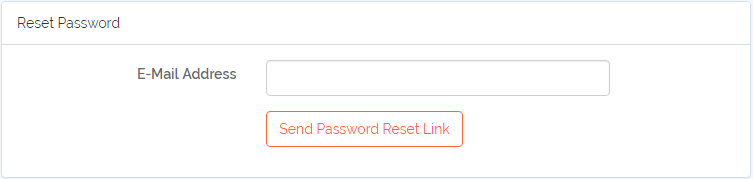
\includegraphics[height=1in]{Images/Implementation/PasswordReset}
\caption{Account recovery page}
\label{fig:PasswordReset}
\end{figure}

\subsection{Widgets}
Widgets are standalone components which are composed of a class and a view. The class is responsible for all the logic and data for the widget and the view is responsible for displaying this data. Parameters may optionally be passed to widgets and can be accessed in the \textit{run()} function of the class. The entire base functionality is provided by a composer package which was included in the project \cite{Packagist:LaravelWidgets}. The base elements are then extended to create custom widgets. A widget can be displayed in any view using the \textit{@widget()} directive.

\subsubsection{Profile}
The profile widget is a standalone component that display the profile information for a specified user, passed through as the second argument of the \textit{@widget()} directive. This widget is used on two separate pages, the home page, for displaying the logged in users profile, and the followers/following page, for displaying the profile of other users. These can be seen in figure \ref{fig:ProfileWidget}. The former is relatively simple as it simply uses a view to render the users details. The latter however uses slightly more complex for the following/unfollowing button. This button is rendered as a partial as it is also used on the profile page.

\begin{figure}[H]
	\centering
	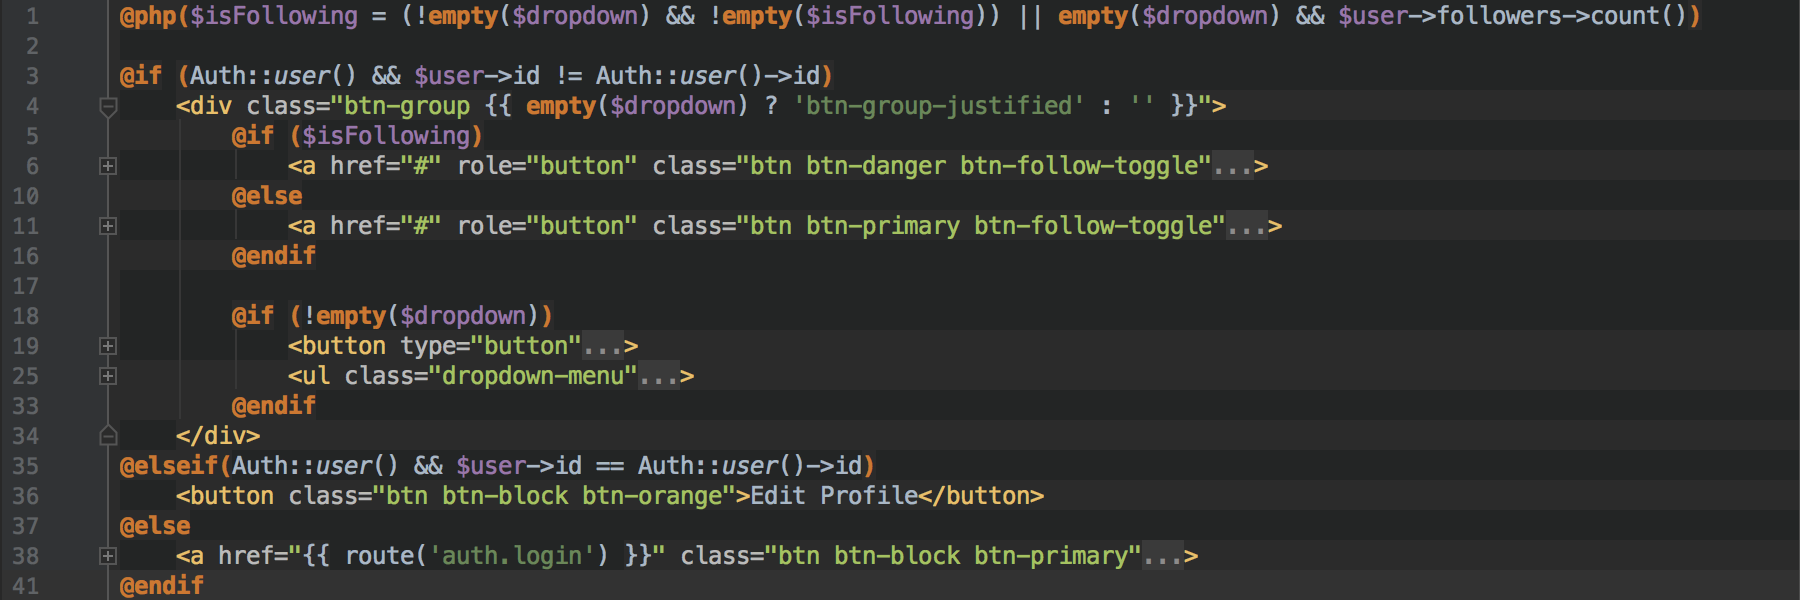
\includegraphics[width=\textwidth]{Images/Implementation/UI/Widgets/Profile_Follow}
	\caption{The code for switching the interactive button on the profile widget.}
	\label{fig:Profile_Follow}
\end{figure}

In order to display the button, we need to first determine the current relationship between the user. This is done using the logic on the first line of figure \ref{fig:Profile_Follow}. The HTML has been collapsed, which hides some of the less important code and PHP logic. Next, if we have an authorised user and this widget is not rendering the same user then we can display the follow or unfollow button based on the relationship. If the dropdown parameter has been defined as true then we add additional options such as block and unblock. If the user is viewing their own profile then we add an edit profile button but this will only occur on the profile page.

\subsubsection{Trending}
\subsubsection{Recommendations}

\subsection{Home}
\subsection{Discover}
\subsection{Notifications}
Figure \ref{fig:NotificationsPage} shows the implemented notifications page. Users receive a notification whenever they receive a new follow, are mentioned in a post by another user, or one of their posts is commented or voted on. The page provides users with information on the notification type, and if relevant the content of the notification (for example, the comment made on their post). The counter, seen next to the bell icon on the navigation bar, indicates to the user how many unread notifications they have. The notification page only fetches unread notifications, which reduces the amount of data that is retrieved from the database. This speeds up the load time of the page. When the user visits the notifications page, all unread notifications are marked as read. 

\begin{figure}[H]
\centering
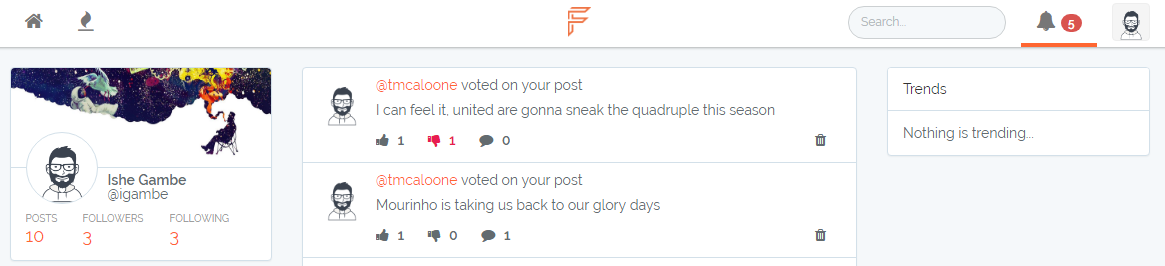
\includegraphics[width=\textwidth]{Images/Implementation/NotificationsPage}
\caption{Notifications Page}
\label{fig:NotificationsPage}
\end{figure}

Laravel provides support for integrating a notification system with your application \cite{Laravel:Notifications}. With this, it is possible to create different notification types, and have these related to a user by using the \texttt{Notification} facade. Using this facade means that whenever an interaction happens with a user or with their posts, they can be notified of this using the \textit{notify()} function:

\begin{lstlisting}[language=bash]
	$user->notify(new NameOfNotification($notification)
\end{lstlisting}

 It is also possible to queue notifications. Creating a queue of notifications can speed up application response time as there can be delays when delivering notifications to the user \cite{Laravel:Notifications, Laravel:Queues}. Queueing can be enabled by adding the \textit{Queueable} trait to the notification class, and starting a queue worker by configuring the queue in \textit{config/queue.php}. Figure \ref{fig:CommentNotification} shows the notification class created for comments. The \texttt{toArray()} function contains an array that represents information carried by the notification. In the array we have a 'regarding' entry, which represents the item the notification is related to, a 'to' entry which represents who the notification is meant for, and a 'text' field which contains information displayed to the user receiving the notification.

\begin{figure}[H]
\centering
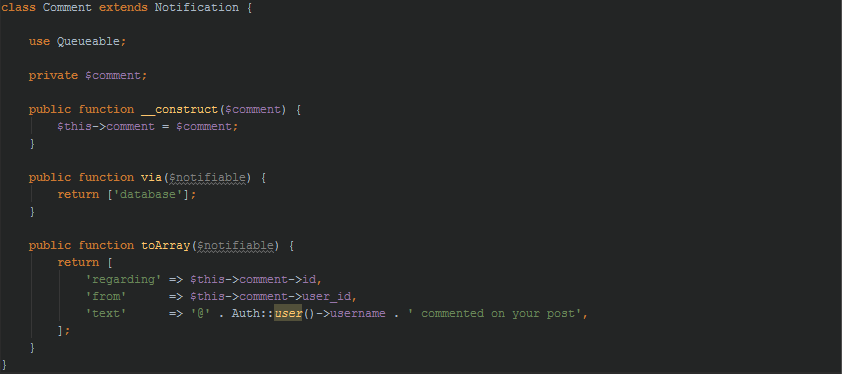
\includegraphics[width=\textwidth]{Images/Implementation/CommentNotification}
\caption{Custom notification for comments}
\label{fig:CommentNotification}
\end{figure}

\subsection{Profile}
\subsection{Settings}
Figure \ref{fig:SettingsImplementation} shows the settings page that allows the user to toggle user account settings. The user is able to modify profile and privacy \& safety settings. In addition to this, they can also manage tags they are subscribed to, and user accounts they have blocked.

\begin{figure}[H]
\centering
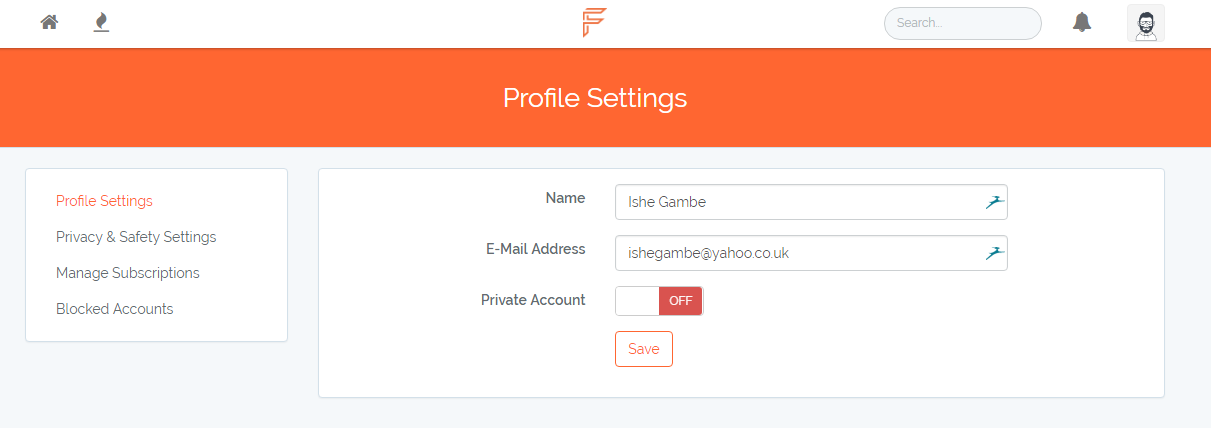
\includegraphics[width=\textwidth]{Images/Implementation/SettingsPage}
\caption{Profile settings from the settings page}
\label{fig:SettingsImplementation}
\end{figure}

Each subset of settings is handled by different controllers. The \textit{AccountController} handles any changes made by the user to their name, email address or the privacy of the account. The controller also handles requests made by the user to edit or upload their profile pictures. The \textit{SafetyController}, seen in Figure \ref{fig:SafetyController}, retrieves the users default settings. As mentioned previously, users are able to modify settings related to abuse detection and recommendations. Before a user has had the chance to modify these settings, default settings are are provided for each user. Default settings are retrieved using the query shown in figure \ref{fig:UserDefaultSettings}. This query is added as a function on the model.

\begin{figure}[H]
\centering
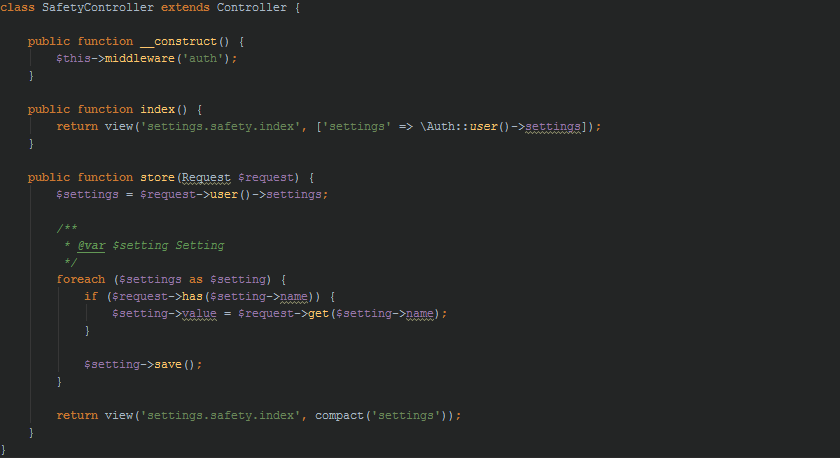
\includegraphics[width=\textwidth]{Images/Implementation/SafetyController}
\caption{Safety Controller}
\label{fig:SafetyController}
\end{figure}

The \textit{SubscriptionsController} returns the users subscriptions in a similar fashion to how default settings are retrieved. The \textit{BlockedController} also follows this approach, using a query to retrieve blocked users defined on the user model to return any blocked users.

\begin{figure}[H]
\centering
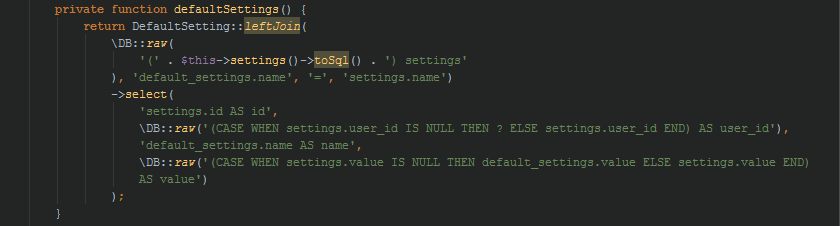
\includegraphics[width=\textwidth]{Images/Implementation/UserDefaultSettings}
\caption{Query to retrieve default settings for the user}
\label{fig:UserDefaultSettings}
\end{figure}

\subsection{Static Pages}
\subsubsection{Privacy Policy}
\subsubsection{Support}